\documentclass[11pt,letterpaper]{article}
\usepackage{naaclhlt2015}
\usepackage{times}
\usepackage{latexsym}
\usepackage{url}
\usepackage[pdftex]{graphicx}
\usepackage{breqn}
\setlength\titlebox{6.5cm}    % Expanding the titlebox

%%%%%%%%%%%%%%%%%%%%%%%%%%%%%%%%%%%%%%%%%%%%%%%%%%%%%%%%%%%%%%%%%%%%%%
% Code to use with NAACL/ACL style files to simulate natbib's 
% \citealt, which prints citations with no parentheses. This should
% work if pasted into the preamble. \cite, \newcite, and \shortcite
% should continue to work as before.

\makeatletter

\def\citealt{\def\citename##1{{\frenchspacing##1} }\@internalcitec}

\def\@citexc[#1]#2{\if@filesw\immediate\write\@auxout{\string\citation{#2}}\fi
  \def\@citea{}\@citealt{\@for\@citeb:=#2\do
    {\@citea\def\@citea{;\penalty\@m\ }\@ifundefined
       {b@\@citeb}{{\bf ?}\@warning
       {Citation `\@citeb' on page \thepage \space undefined}}%
{\csname b@\@citeb\endcsname}}}{#1}}

\def\@internalcitec{\@ifnextchar [{\@tempswatrue\@citexc}{\@tempswafalse\@citexc[]}}

\def\@citealt#1#2{{#1\if@tempswa, #2\fi}}

\makeatother
%%%%%%%%%%%%%%%%%%%%%%%%%%%%%%%%%%%%%%%%%%%%%%%%%%%%%%%%%%%%%%%%%%%%%%

% Effects of non-linguistic context
\title{Shared common ground influences information density in microblog texts\Thanks{Thanks to...}}
% common ground decreases information

\author{Author 1\\
XYZ Company\\
111 Anywhere Street\\
Mytown, NY 10000, USA\\
{\tt author1@xyz.org}
	  \And
          Author 2\\
ABC University\\
900 Main Street\\
Ourcity, PQ, Canada A1A 1T2\\
{\tt author2@abc.ca}
}

\date{}


\begin{document}
\maketitle
\begin{abstract}
Natural languages offer many possible ways to say the same thing. If speakers use language rationally, they should structure their messages to achieve approximately uniform information density (UID), in order to maximize transmission via a noisy channel. Previous work identified a consistent increase in linguistic information across sentences in text as a signature of the UID hypothesis. This increase was derived from a predicted increase in context, but the context itself was not quantified. We use microblog texts from Twitter, tied to a single shared event (the baseball World Series), to quantify contextual information. By tracking changes in contextual information, we identify both gradual and rapid changes in information content in response to in-game events. These findings lend further support to the UID hypothesis and highlights the importance of non-linguistic common ground for language production and processing.
\end{abstract}

\section{Introduction}

Natural language is an incredibly powerful method for representing and communicating information. One consequence of this power is that there is an infinity of different ways to structure any particular message. How do speakers choose between different possible structures? One provocative hypothesis is that they attempt to structure their message to best convey their intended meaning in the context of their communication. On this view, the use of natural languages is assumed to follow optimal information transmission results from information theory \cite{shannon1948}. In particular, speakers should structure their messages to approximate \emph{uniform information density} across symbols (words and phonemes), which is optimal for transmission of information through a noisy channel. 

At least three lines of evidence suggest that speakers do make choices to increase the uniformity of information density across their utterances. First, speakers phonologically reduce more predictable material \cite{aylett2004,aylett2006,bell2003}. Second, they omit or reduce optional lexical material in cases where the subsequent syntactic information is relatively more predictable \cite{levy2007,frank2008,jaeger2010}. Third, and most relevant to our current hypothesis, speakers appear to increase the complexity of their utterances as a discourse develops \cite{genzel2002,genzel2003,qian2012}. We expand on this finding below.

Following the UID hypothesis, \citealt{genzel2002} proposed that $H(Y_i)$, the total entropy of part $i$ of a message (e.g., a word) is constant. They compute this expression by considering $X_i$, the random variable representing the precise word that will appear at position $i$, conditioned on all the previous observed words. They then further factor this expression into two terms:\vspace*{-1.5em}

\begin{eqnarray}
H(Y_i) &=& H(X_i | C_i, L_i) \\
&=& H(X_i | L_i) - I(X_i ; C_i | L_i) \label{eq:gc}
\end{eqnarray}

\noindent where the first term $H(X_i | L_i)$ is the dependence of the current word on only the local linguistic context (e.g. within the rest of the sentence $L_i$) and the second is the mutual information between the current word and the broader linguistic context $C_i$, given the rest of the current sentence. On their logic, with greater amounts of contextual information, the predictability of linguistic material based on context, $I(X_i | C_i, L_i)$ must go up. Therefore, they predicted that $H(X_i|L_i)$ should also increase, so as to result in a constant total amount of information. 

% For convenience, we rewrite Equation \ref{eq:gc} as

% \begin{equation}
% \label{eq:lambda}
% H(X_i | L_i) - I(X_i ; C_i | L_i) = \lambda
% \end{equation}

% \noindent where $\lambda$ is a constant. 

Genzel and Charniak then approximated $H(X_i | L_i)$ using a number of methods and showed that it did increase systematically in documents. Later work showed that this increase was strongest within paragraphs and was general across document types \cite{genzel2003} and languages \cite{qian2012}. No attempt was made in this work, however, to measure shared context (and its influence on message expectations) directly. This challenge is the focus of our current work. 

\subsection{Contextual effects on complexity}

In psycholinguistics, the notion of shared \emph{common ground} is a more precise replacement for the general notion of ``context'' \cite{clark1996}. Common ground is defined as the knowledge that participants in a discourse have and that participants know other participants have, including the current conversational context beyond the specific language that is used. A large literature supports the idea that speakers consider referential context and other linguistic common ground in selecting the appropriate expression to refer to a particular physical object \cite{brennan1996,metzing2003,dale1995,sedivy1999}. In principle, Genzel and Charniak's formulation can be considered as capturing the relationship between all of shared common ground---both linguistic and non-linguistic---and the predictability of language, even though in that previous work only linguistic information was considered. 

When there is both linguistic and non-linguistic information passing through the channel, both information streams are passing through a noisy channel, so the relevant quantity is not the marginal entropy of only the linguistic stream but the joint entropy of both streams.  Let $T_j$ be the linguistic information in part $j$ of the discourse, and $E_j$ be the non-linguistic information in part $j$.  If $C_j$ is the built-up context from the preceding parts $\{1,\cdots,j-1\}$ of the discourse, then we can break down the joint entropy as:\vspace*{-1.5em}

% \begin{dgroup}
%   \begin{dmath}
%     H(T_j,E_j|C_{j-1}) = H(T_j|E_j,C_{j-1}) + H(E_j|C_{j-1})  
%   \end{dmath}
%   \begin{dmath*}
%     = H(T_j|C_{j-1}) - I(T_j;E_j|C_{j-1}) + H(E_j|C_{j-1}) 
%   \end{dmath*}
%   \begin{dmath*}
%    = H(T_j) - I(T_j;C_{j-1}) - I(T_j;E_j|C_{j-1}) + H(E_j|C_{j-1}) 
%   \end{dmath*}
%   \begin{dsuspend}
%     Which can be reduced to:
%   \end{dsuspend}
%   \begin{dmath}
%     \label{eq:joint-entropy}  H(T_j) - I(T_j;E_j,C_{j-1})  + H(E_j|C_{j-1})
%   \end{dmath}
% \end{dgroup}


\begin{eqnarray}
\nonumber &&\hspace*{-2.5em}H(T_j,E_j|C_{j-1}) \\
\nonumber &=& H(T_j|E_j,C_{j-1}) + H(E_j|C_{j-1}) \\
\nonumber                    &=& H(T_j|C_{j-1}) - I(T_j;E_j|C_{j-1}) + H(E_j|C_{j-1}) \\
\nonumber                    &=& H(T_j) - I(T_j;C_{j-1}) \\
\nonumber                    && \quad - I(T_j;E_j|C_{j-1}) + H(E_j|C_{j-1}) \\
\label{eq:joint-entropy}     &=& H(T_j) - I(T_j;E_j,C_{j-1}) + H(E_j|C_{j-1})
\end{eqnarray}

By the UID hypothesis, we expect the left-hand side of this equation to be constant, as it is the information content of each part of the discourse.  The first term of the right-hand side is the out-of-context entropy of the linguistic information. The second term is the mutual information of the linguistic information and the union of the preceding context plus the current non-linguistic information (the events occurring at the time).  The third term is the entropy of the non-linguistic information, given the preceding context.

This breakdown suggests that rational participants in a discourse will exhibit both slow and fast adaptation to context in order to maintain overall constant entropy.  As context slowly builds, the mutual information term grows (and the non-linguistic entropy likely shrinks), resulting in the time-based increase in $H(T_j)$ that previous work has found.  In addition, an individual event can have high or low information content given the context, without having a large effect on the mutual information term.  To maintain constant entropy, high-information events should be accompanied by low-information linguistic responses, and vice versa.  With an operationalization of shared context, we should be able to observe these two types of adaptation directly, not just via the increasing trend shown in previous work \cite{genzel2002,qian2012}.  

To test this prediction, we leverage twitter, a popular microblogging service, to operationalize common ground. Because of its structure, twitter is an ideal platform for this investigation. One common method of using twitter is to mark messages with hashtags, which serve as ad-hoc categories, allowing anyone interested in a topic to find the messages relevant to that topic. This strategy is especially used when users are commenting on an external event (e.g. a sporting, media, or political event). We focus here on the World Series of baseball, an annual sporting event with large viewership and a single broadcast stream; in this case, the hashtag is \texttt{\#worldseries}. Hashtagged messages are part of a discourse with extremely limited prior linguistic context, as no two tweeters will have seen the same set of tweets. The total shared context with the audience that can be assumed by the writer of a tweet is the non-linguistic content of the event being hashtagged. 

We begin by describing our corpus and our method of calculating linguistic content (by computing entropy within a simple $n$-gram model). We then investigate gradual changes in word-by-word information content as the event goes on (testing adaptation driven by contextual mutual information in Equation \ref{eq:joint-entropy}, replicating \citealt{genzel2002}) and rapid changes in the total information content of tweets in response to important in-game events (testing adaptation driven by non-linguistic information in Equation \ref{eq:joint-entropy}). We end by considering a number of control analyses that provide evidence against alternative accounts of our results. 

%\subsection{First version of contextual effects}
%
%Although Genzel and Charniak stated the regularity in terms of the current word, an alternative formulation would be in terms of the total information content of the utterance. We can see this by summing Equation \ref{eq:lambda} across words:
%
%\begin{equation}
%H(X) - I(X | C) = |X| \lambda
%\end{equation}
%
%\noindent where $H(X) = \sum_i{H(X_i|L_i)}$ and $I(X|C) = \sum_i{I(X_i | C_i, L_i)}$. Hence,
%
%\begin{equation}
%\label{eq:prop}
%H(X) \propto -I(X|C).
%\end{equation}
%
%\noindent This proportionality indicates that as the amount of shared context goes up, the total linguistic complexity should go down. Thus, if we have an operationalization of shared context, we should be able to observe this proportionality directly, not just via the increasing trend shown in previous work \cite{genzel2002,qian2012}. 
%
%In psycholinguistics, the notion of shared \emph{common ground} is a more precise replacement for the general notion of ``context'' \cite{clark1996}. Common ground defined as constituted the total of knowledge that communicators share with their audience. In particular, a broad literature suggests that speakers consider common ground in selecting the appropriate expression to refer to a particular object \cite{brennan1996,metzing2003}. In principle, Genzel and Charniak's formulation can be considered as capturing the relationship between shared common ground and the predictability of language. 
%
%To test this prediction, we leverage twitter, a popular microblogging service, to operationalize common ground. Because of its structure, twitter is an ideal platform for this investigation. One common method of using twitter is to mark messages with hashtags, which makes them viewable and searchable to the entire twitter audience. This strategy is especially used when users are commenting on an external event (e.g. a sporting, media, or political event). We focus here on the World Series of baseball, an annual sporting event with large viewership; in this case, the hashtag is \texttt{\#worldseries}. Hashtagged messages thus form a case in which there is \emph{no} prior linguistic context. The total shared context with the audience that can be assumed by the writer of a tweet is the non-linguistic content of the event being hashtagged. 
%
%We begin by describing our corpus and our method of calculating linguistic content (by computing entropy within a simple $n$-gram model). We then investigate gradual changes in word-by-word information content as the event goes on (testing Equation \ref{eq:gc}) and rapid changes in the total information content of tweets in response to important in-game events (testing Equation \ref{eq:prop}). We end by considering a number of control analyses that provide evidence against alternative accounts of our results. 

\section{Corpus and Methods}

\subsection{\#Worldseries Corpus}

Our current analysis looked at tweets during the 2014 World Series, a series of seven baseball games in late October 2014.  We obtained these tweets by searching publicly-available tweets through the Twitter API, using an adaptation of SeeTweet \cite{doyle2014} to compile tweets containing the hashtag ``\#WorldSeries.''  To synchronize tweets with game events, we used the Major League Baseball Advance Media XML repository,\footnote{\url{http://gd2.mlb.com/components/game/mlb/}} which contains pitch-by-pitch data including the ongoing state of the game and timestamps at the start of each at-bat. Using this timestamp information, we binned tweets by at-bats so that they could be co-registered with other in-game statistics.  These bins extend from the time of the first pitch in an at-bat to the beginning of the next at-bat, and thus provide time for reactions to the events of the at-bat.\footnote{We tested a series of potential offset times in case Twitter and MLB used different clocks or at-bats were not long enough to capture reactions. We did not adjust the times as there was no significant increase in the correlation between Leverage Index (Sect. \ref{sect:other-metrics}) and tweet rate for these offsets.}  The mean at-bat length was 2.76 minutes, and there were 512 total at-bats.  We limited our analysis to tweets timestamped during one of these at-bats, resulting in a total corpus of 109,207 tweets. Each game had its first pitch at approximately 0008 UTC, and lasted between three and four hours.

Our tweet corpus was compiled from the ``garden-hose'' Twitter search API, which returns a subset of all relevant tweets. Our searches captured approximately 4\% of all relevant tweets; Twitter reported 420,329 relevant tweets during Game 1 of the World Series\footnote{\url{https://twitter.com/TwitterData/status/524972545930301440}}, and our dataset contained 17,538 tweets during the same time period.  We address potential confounds from this sampling process in Section \ref{sect:speaker-normalization}.

\subsection{Entropy Computation}

We estimated the linguistic information content of each tweet in our corpus. Social media text has been described as ``bad language'' \cite{eisenstein2013}: It can be difficult to model due to its idiosyncratic abbreviations, typographic errors, and other non-standard forms. Relevant to our goal of assessing information content, it can also be difficult to create an appropriate training corpus for language models, since the vocabulary and composition of tweets of change rapidly \cite{eisenstein2013}.

We attempted to minimize these difficulties in two ways.  First, we estimated language models with domain-specific corpora. In particular, for tweets from each game we used a training corpus consisting of the tweets from all the other games. This training set provided a vocabulary and structure that was similar in topic and style and to the test set.  We removed all punctuation and emoji except word-initial {\it @} and {\it \#}, which refer to users and hashtags, respectively.  Usernames were replaced with {\it [MENTION]} to reduce sparsity; hashtags were not altered, as these often function as words or phrases within the tweet's syntax.  Words with fewer than 5 occurrences in the training corpus were marked as out-of-vocabulary items. We estimated trigram models using a modification of NLTK \cite{bird2006}\footnote{Smoothing on n-gram models in NLTK can be inaccurate (see \url{https://github.com/nltk/nltk/issues/367}), so we used a modified version courtesy of B. C. Roy (personal communication).} with Witten-Bell smoothing, and estimated per-word and total entropy for each tweet from these models.

Second, we included tweet length (in characters) as an alternative metric of information content (see Section \ref{sect:speaker-normalization}). Unless information rate varies systematically across tweets of different lengths---counter to the claim of approximately uniform information density in language \cite{genzel2002,levy2007}---longer tweets will generally carry more information. 


\section{Gradual Changes in Information Rate}

Our first analytic goal was to examine changes in the information content of tweets due to the long-term build-up of context in a shared event.  We predicted that we would see similar developments in information structure as in more traditional conversational settings, even though there was no formal conversation or explicit linguistic history to develop common ground.  Specifically, we predicted that the build-up of contextual information would cause the context-independent per-word entropy to rise over time, replicating the effect that has been observed across languages and genres \cite{genzel2002,genzel2003,qian2012}.

\begin{figure}
 \centering
  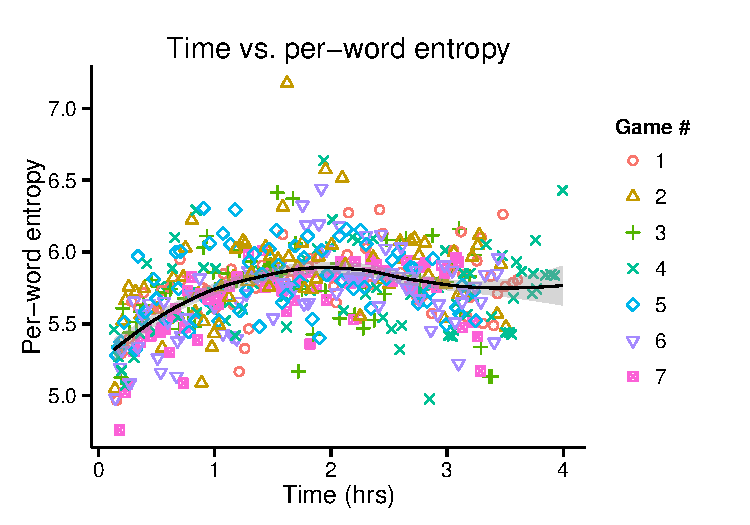
\includegraphics[width=3.25in]{figures/fig1.pdf}
 \caption{Per-word entropy increases with time for the first two hours of the games, then levels off and slightly declines. Color reflects in-game time; line shows loess fit with 95\% confidence intervals.}\label{fig:time-perword-ent}\vspace*{-.5em}
\end{figure}

\begin{table*}
  \begin{tabular}{clc}
 Minute & Tweet & Per-word entropy \\
\hline
0 & \#WorldSeries Play Ball & 4.96\\
0 & It's finally here! \#WorldSeries & 4.74\\
0 & \parbox[][6ex][c]{.7\textwidth}{IDEA: @mayoredlee, \#SanFrancisco can pledge to throw our @SFGiants an \#OrangeOctober parade regardless of \#WorldSeries outcome! \#SFGiants} & 8.20\\
\hline
12 & The guy with the Marlins sweater is behind home plate again. \#worldseries & 4.26\\
12 & \parbox[][6ex][c]{.7\textwidth}{Something about Hunter Pence really, really bothers me. Don't ask me what, cause I havent figured it out, but I don't like him. \#WorldSeries} & 6.64\\
12 & The Giants 3-0! \#WorldSeries & 5.43\\
\hline
73 & \parbox[][6ex][c]{.7\textwidth}{Three HORRIBLE at-bats (mixed in with Cain's walk) prevent Royals from breaking through in the third. \#WorldSeries} & 9.39\\
130 & \parbox[][6ex][c]{.7\textwidth}{As Hardy Boy \#2, Joe Panik just pulled the mask off of Vargas and discovered it's Old Man Withers from down the street. \#WorldSeries} & 8.12\\
178 & \parbox[][6ex][c]{.7\textwidth}{\#WorldSeries it's funny the non body names have a great hits. Frm now n on consider the Postseson as Cinderla run.  No names needed, \#MLB} & 10.04\\
\hline
  \end{tabular}
 \caption{Example tweets, grouped by minutes since the first pitch.}\label{tab:ex}
\end{table*}

Figure \ref{fig:time-perword-ent} shows evidence for changes in per-word entropy over the course of games. Per-word entropy rises sharply in the first half-hour of each game, then begins to level off and finally declines slightly over time.  This pattern is consistent with the constant entropy rate proposal of \cite{genzel2002}, and more specifically with the context decay model of \citealt{qian2012}.\footnote{A late decline in per-word entropy also appeared in \citealt{qian2012}'s analysis of Swedish.} 

We used mixed-effects linear regression to quantify this relationship, using the time of an at-bat to predict both per-word and per-tweet entropy during the at-bat. Specifically, we used the logarithm of time as our fixed-effect predictor, per the context-decay models of \cite{qian2012}.  We added game-specific random intercepts and slopes of log-time to capture cross-game variation. This model showed significant positive effects of time on entropy, using likelihood-ratio tests for both models (per-word entropy: $.348 \pm .045; p<.001, \chi^2(3)=104.6$, per-tweet entropy: $10.31 \pm 2.08; p=.001, \chi^2(3)=74.65$). %Significant positive effects of time on entropy are found through likelihood-ratio tests for both models (per-word: $.080 \pm .016; p<.001, \chi^2(1)=11.02$, per-tweet: $2.61 \pm .74; p=.008, \chi^2(1)=7.12$).

We hypothesize that this finding---greater linguistic entropy for later tweets---is due to the accrual of common ground across users from shared non-linguistic information. As they watch more of the game, they share more referents and have stronger expectations about what aspects of the game will be discussed. This shared common ground licenses more complex language and more sophisticated linguistic references. Table \ref{tab:ex} gives example tweets at different time points; as a game progresses, references can expand from generic references to the teams or series, to specific individuals and events, and eventually to sequences of events.

While this finding is consistent with previous work on the effect of context \cite{genzel2002,qian2012}, it expands the definition of context.  In previous work, the context came from explicit linguistic information built up through paragraphs in a formally-structured, written document.  In the Twitter dataset, the context comes from real-world events during the games, as there is no canonical shared sequence of tweets that the tweeters can refer back to (indeed, two random users of the \#Worldseries hashtag probably have relatively little twitter context in common).  In sum, contextual influences on entropy need not be explicitly linguistic, so long as discourse participants have reason to believe that the other participants share their knowledge.

\section{Fast Changes In Information Content}

\begin{figure}
 \centering
  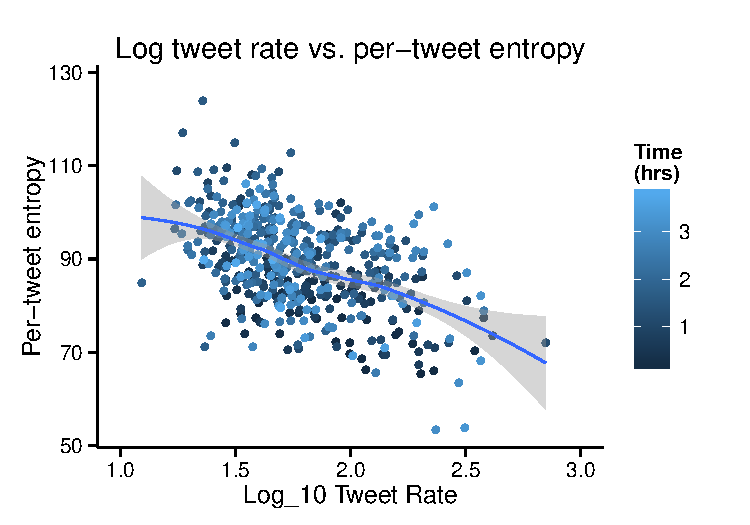
\includegraphics[width=3.25in]{figures/fig2.pdf}
 \caption{Total tweet entropy plotted against log tweet rate. Color reflects in-game time; line shows loess fit with 95\% confidence intervals.}\label{fig:lrate-tent}\vspace*{-.5em}
\end{figure}

\begin{table*}
  \begin{tabular}{clc}
Log rate & Tweet & Per-word entropy \\
%\hline
%2.61 & Butler channeled his inner "The Little Engine That Could" running the bases! \#Royals \#Game7 \#WorldSeries & 6.30\\
%2.61 & Was \#Butler Running Is Slo-Mo!!! \#WorldSeries \#Game7 & 8.16\\
%2.61 & Aside from chasing after a food truck, I don't think I've ever seen Billy Butler run that fast! Hang tough, \#KC! \#WorldSeries \#Royals & 7.70\\
\hline
2.49 & Fuck you, Blanco. \#Giants \#WorldSeries & 5.54\\
2.49 & Holy shitballs, @Royals! \#WorldSeries \#Game7 & 3.99\\
2.49 & Just when you thought the \#WorldSeries was over.... \#E8 & 4.76\\
\hline
1.66 & \parbox[][6ex][c]{.7\textwidth}{I suppose I appreciate Bochy's ``ASG'' approach with Bumgarner. Of course, who are any of us to question him in late October? \#WorldSeries} & 7.42\\[3pt]
1.66 & \parbox[][6ex][c]{.7\textwidth}{The guy in Marlins gear behind home plate needs to escorted off property for annoying everybody. \#WorldSeries \#WhoDoesThat} & 4.85\\[3pt]
1.66 & Lets Go Giants!!! 5-0  \#SFGiants \#WorldSeries & 3.26\\
\hline
  \end{tabular}
 \caption{Example tweets, grouped by the per-minute tweet rate during each at-bat.}\label{tab:ex2}
\end{table*}

Intuitively, after an exciting, game-changing event, tweets will be shorter and make more reference to the shared knowledge that this event has just happened. Such events should also generate more responses, suggesting that the number of tweets per unit time can serve as a proxy for the information content of an event. This relationship is captured by Equation \ref{eq:joint-entropy}, in which unexpected events have large information content and linguistic information content should be reduced correspondingly to maintain constant entropy. Our next set of analyses test this relationship. 

The examples shown in Table \ref{tab:ex2} provide anecdotal evidence for the hypothesized relationship between in-game events and linguistic complexity, with examples of consecutive tweets from high-rate and low-rate at-bats, along with their information content. The top triplet comes from one of the highest-rate at-bats, in which Gregor Blanco committed a crucial error in the last inning of the last game.  The bottom triplet comes from a low-rate at-bat, mid-game in a developing blowout\footnote{Blowouts are games whose outcome is easy to predict relatively early.}; in this case, tweets all refer to different events as there is no single salient shared event.

%This short-timescale adaptation is predicted for two reasons. First, it represents a rational response to issues of information overload, the state where the amount of incoming information exceeds a user's ability to process it \cite{miller1956}.  Previous investigations into online forum posting behavior have shown such rational responses on a longer timescale \cite{jones2001a,jones2001b,whittaker2003,schoberth2003}, as well as the more explicitly conversational setting of IRC chat channels \cite{jones2008}.  Second, given that the hashtagged tweets are tied to an ongoing real-world event, changes in tweet rates are likely to be tied to what is happening in the event, providing a potential proxy for the non-linguistic context available at the time of the tweet. We will expand on this second explanation in Section laden\ref{sect:other-metrics}.

We quantified the predicted relationship by again fitting a mixed-effect linear regression model, in this case using the logarithm of per-minute tweet rate as a predictor of tweet entropy.  Given its significance in the previous model, we included log(time) as a control factor in this analysis, and added by-game random intercepts and slopes for log(rate) and log(time).  The log of the tweet rate had a significant negative effect on per-word and per-tweet entropy by likelihood-ratio tests (per-word-entropy: $-.333 \pm .073; p<.001, \chi^2(4)=59.37$, per-tweet-entropy: $-21.82 \pm 2.43; p<.001, \chi^2(4)=194.6$). 

Log(time) retained significance ($p<.001$) as a predictor for both entropy measures even when rate was accounted for, showing evidence for both slow and fast adaptation occurring in the discourse.  The effects are both in the predicted directions: Entropy increases with time as more informative context builds up, but decreases with tweet rate as more exciting events encourage less information-laden tweets.

\section{Control Analyses}

\subsection{Non-Rate Metrics of Context}\label{sect:other-metrics}

Since tweet rate is an organic reflection of the interest accrued by in-game events, it is an important metric for examining fast adaptation. Nevertheless, it could be confounded with other factors influencing tweet production.  For instance, there is evidence that online interactions exhibit rational responses to information overload, the state where the amount of incoming information exceeds a user's ability to process it \cite{miller1956,schoberth2003}.  Previous investigations into forum posting behavior have shown that users adapt to overload by posting shorter messages \cite{jones2001a,jones2001b,whittaker2003,schoberth2003}, and a similar result was found for the more explicitly conversational setting of IRC chat channels \cite{jones2008}.   

To show that the changes in information content are not merely reactions to increased tweet competition---that they have independent informational motivations---we need metrics of event importance and predictability that are not dependent on social media behavior.  Luckily, baseball has a long history of statistical analysis, and as a result, there are independently-derived metrics that fit this bill.  Two that are appropriate for this purpose are {\it Leverage Index} (LI)\footnote{\url{http://www.hardballtimes.com/crucial-situations/}} and  {\it Win Probability Added} (WPA) \cite{tango2007}.


\begin{figure}
 \centering
  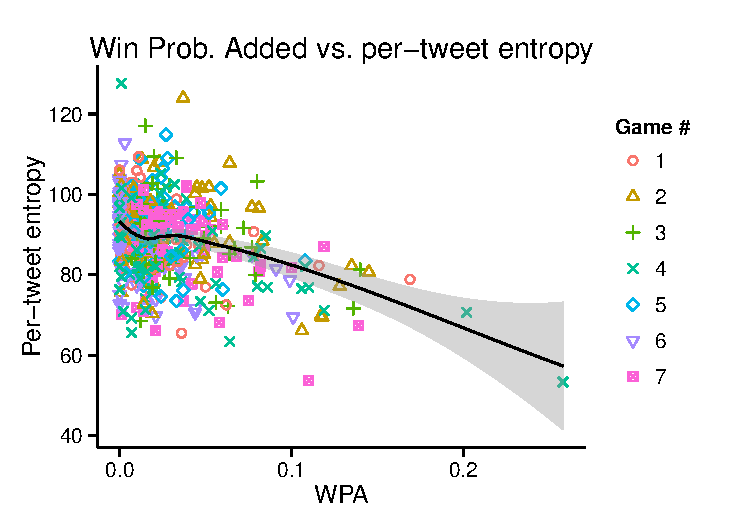
\includegraphics[width=3.25in]{figures/fig3.pdf}
 \caption{Total entropy decreases for at-bats with greater win probability changes. Loess curve fitting with 95\% confidence intervals.}\label{fig:wpa-tent-agg}\vspace*{-.5em}
\end{figure}

% To show that the changes in information content are not merely reactions to increased tweet competition but have independent informational motivations, we need metrics of event importance and predictability that are not dependent on social media behavior.  Baseball has a long history of statistical analysis, and as a result, there are independently-derived metrics that fit this bill.  Two that are appropriate for this purpose are {\it Leverage Index} (LI)\footnote{\url{http://www.hardballtimes.com/crucial-situations/}} and  {\it Win Probability Added} (WPA) \cite{tango2007}.

LI is an estimate of how critical an at-bat is to the outcome of the game.  It is based on the difference in resultant win probability if the current batter gets a hit or an out, normalized by the mean change in win probability over all at-bats. 1 is the average LI, and greater LI indicates greater importance.  LI, as a measure of the expected change in win probability, is similar to non-linguistic entropy term in Equation \ref{eq:joint-entropy}.  In contrast, WPA depends on the result of an at-bat, and estimates how much the win probability changed as a result of what happened during the at-bat.  WPA thus provides an estimate of how much information about the game outcome this at-bat has provided, conditioned on the current game context.  These measures are well-correlated (Kendall's $\tau=.77$), since a high-LI at-bat's value comes from its ability to affect win probability.

As high LI or WPA values indicate an at-bat whose result has a large effect on the game, these metrics provide an estimate for non-linguistic informativity that is independent of medium-specific influences on tweet production.  To assess their effects, we constructed four mixed-effects linear regression models, using LI and WPA to predict per-word and per-tweet entropy in all pairwise combinations (we built separate models for LI and WPA due to their high collinearity). Fixed- and by-game random-effects of log(time) and log(rate) were included as controls in all models; if there is an effect of LI or WPA beyond the effect of rate, this effect can be interpreted as evidence of speaker adaptation to non-linguistic information content.

Both LI and WPA had significant negative effects on per-tweet entropy (LI: $-1.52 \pm .43; p=.001, \chi^2(5)=20.1$, WPA: $-2.27 \pm .40; p<.001, \chi^2(5)=44.18$), over and above the effect of tweet rate.  Per-word entropy did not show a significant effect of LI or WPA when rate was included as a control factor. Each was a significant factor on per-word entropy ($p=.008,p=.005$) when rate was not included as a control, though, suggesting that the explanatory power of these independent metrics may be subsumed in the more complex factor of tweet rate.

\subsection{Speaker Normalization}
\label{sect:speaker-normalization}

A second alternative hypothesis for the observed behavioral changes with tweet rate is that they arise not from changes in the behavior of individuals but rather from a change in demographics.  It is plausible that rising tweet rates come from an influx of new tweeters using the hashtag, and that these new tweeters simply produce shorter, less informative tweets in general.  For instance, spambots often include trending hashtags in their spam tweets \cite{martinez2013}. To account for this, we treated the users whose tweets are in our corpus as a ``computational focus group'' \cite{lin2013,lin2014}, and used the Twitter API to collected a further 100 tweets from each user outside the timeframe of the games.  We used these tweets to estimate an average tweet length for each user, and subtracted this value from the length of their \#worldseries tweets during the games.\footnote{Note that these analyses are conducted over tweet length, rather than total entropy, as there was no obvious way of normalizing entropy by speaker.} If this baselined metric displays the same effects as shown above, we have reason to believe that users are in fact changing their individual behaviors in response to information factors, rather than that a demographic shift is mimicking a behavioral shift.

\begin{figure}
 \centering
  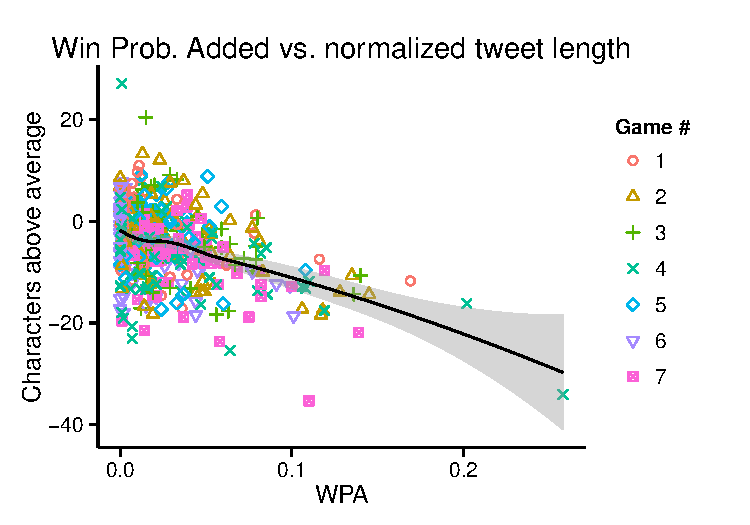
\includegraphics[width=3.25in]{figures/fig4.pdf}
 \caption{Speaker-normalized tweet length also decreases for at-bats with greater win probability changes. Loess curve fitting with 95\% confidence intervals.}\label{fig:wpa-ld-agg}\vspace*{-.5em}
\end{figure}

For this analysis, we created a mixed-effects model with WPA, log(rate) and log(time) as predictors of tweet length.  All three factors were significant (WPA: $-1.64 \pm .36; p<.001, \chi^2(5)=72.3$; log(rate): $-6.15 \pm .47; p<.001, \chi^2(5) =303.6 $; log(time): $.82 \pm .40; p=.001, \chi^2(5)=20.6$).  We then created a second model using the same factors to predict the mean change in tweet length from the baseline length. Again, all three factors were significant (WPA: $-2.01 \pm .29; p<.001, \chi^2(5)=70.2$; log(rate): $-5.10 \pm .49; p<.001, \chi^2(5) = 252.6$; log(time): $.61 \pm .35; p=.016, \chi^2(5)=14.0$).  By ruling out demographic shifts (e.g. an influx of terser tweeters using the hashtag), this analysis provides additional support for the idea that tweeters indeed shift their behavior in response to in-game information.

\section{Discussion}

We investigated the hypothesis that speakers optimize their language production so as to approximate \emph{uniform information density}, a signature of efficient communication through a noisy channel \cite{shannon1948,levy2007}. Previous work had observed indirect evidence for UID via increases in linguistic complexity (which were hypothesized to reflect increasing discourse/contextual knowledge), but this work neither measured contextual information directly nor included non-linguistic measures of context \cite{genzel2002,genzel2003,qian2012}. Our current work takes a first step towards addressing these issues by using microblog texts around shared events (baseball games) as a case study in which a known context can be characterized more precisely. With this approach, we find systematic differences in information rate and total information content as a function of nonlinguistic factors. 

We successfully replicated the effect found in previous work: a gradual increase in entropy rate over the course of individual baseball games. But in addition to this effect, we found a striking pattern of short-timescale changes in total message entropy (reflected in the changing lengths of messages). When in-game events were exciting, unpredictable, and outcome-relevant (hence, highly informative), message length and total entropy went down. This regularity suggests that twitter users were regulating the information content of their messages relative to the total communicative content of the context more broadly, a prediction that can be derived directly from the UID model. 

Our work highlights the importance of non-linguistic context for the informational content of language. This relationship is widely acknowledged in theories of pragmatic communication \cite{grice1975,sperber1986,clark1996,frank2012}, but has been largely absent in information-theoretic treatments of linguistic complexity. The omission of this information has largely been for pragmatic, rather than theoretical, reasons: As \citealt{genzel2002} note, it is typically very difficult to compute semantic---let alone non-linguistic---information content. Our work suggests that internet communications surrounding shared media events may be a promising source of grounded language use where context can be quantified more effectively due to the existence of substantial metadata. 

A growing literature suggests that the information content of language is the critical variable for understanding processing difficulty in language comprehension \cite{levy2008,demberg2008,boston2008,smith2013}. Under surprisal theory \cite{hale2001,levy2008}, the overall predictability of individual elements of language is assumed to be due to a predictive model of its likelihood in the current context. Given this model of processing difficulty, our work here makes a strong prediction: that the information processing difficulty of a word or sentence should track with its total information content (including its relationship to the non-linguistic context), rather than its linguistic information content alone. Some preliminary evidence supports this idea. In a study of the processing complexity of negative utterances, \citealt{nordmeyer2014} found that the processing cost of negation was predicted by the surprisal of the negation in a particular pragmatic context. But future work should test this hypothesis across a wider variety of structures and contexts. 

In sum, our work contributes to the growing body of evidence in favor of the UID hypothesis. The mechanisms underlying the tendency to regulate information content are still unknown, however. While UID would follow from a strong form of \emph{audience design}, in which speakers explicitly consider the processing difficulty of different content \cite{clark1996}, the UID hypothesis could also emerge from simpler production processes. Untangling these possibilities will not be trivial. Regardless of the resolution of this issue, however, UID appears to be an important descriptive tool in capturing how speakers make production choices. 

%\section*{Acknowledgments}
%
%We gratefully acknowledge the support of ONR Grant N00014-13-1-0287.

\newpage

\bibliographystyle{naaclhlt2015}
\bibliography{tweetprag}

\end{document}